\begin{figure}[!h]
    \centering
    \begin{subfigure}{.5\textwidth}
      \centering
      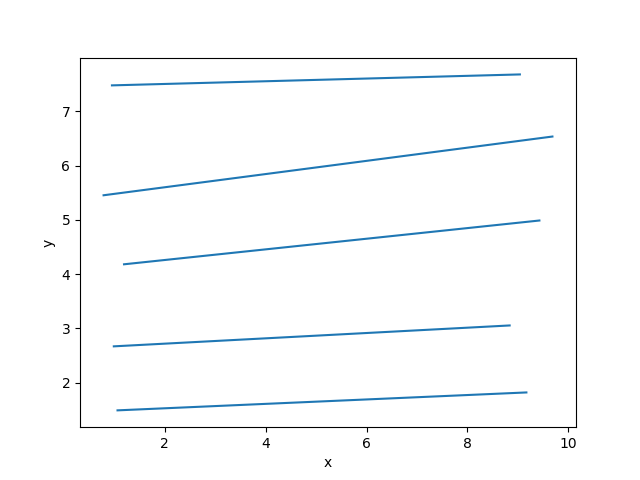
\includegraphics[width=.9\linewidth]{0.png}
      \caption*{Rys. 1}
      \label{fig:sub1}
    \end{subfigure}%
    \begin{subfigure}{.5\textwidth}
      \centering
      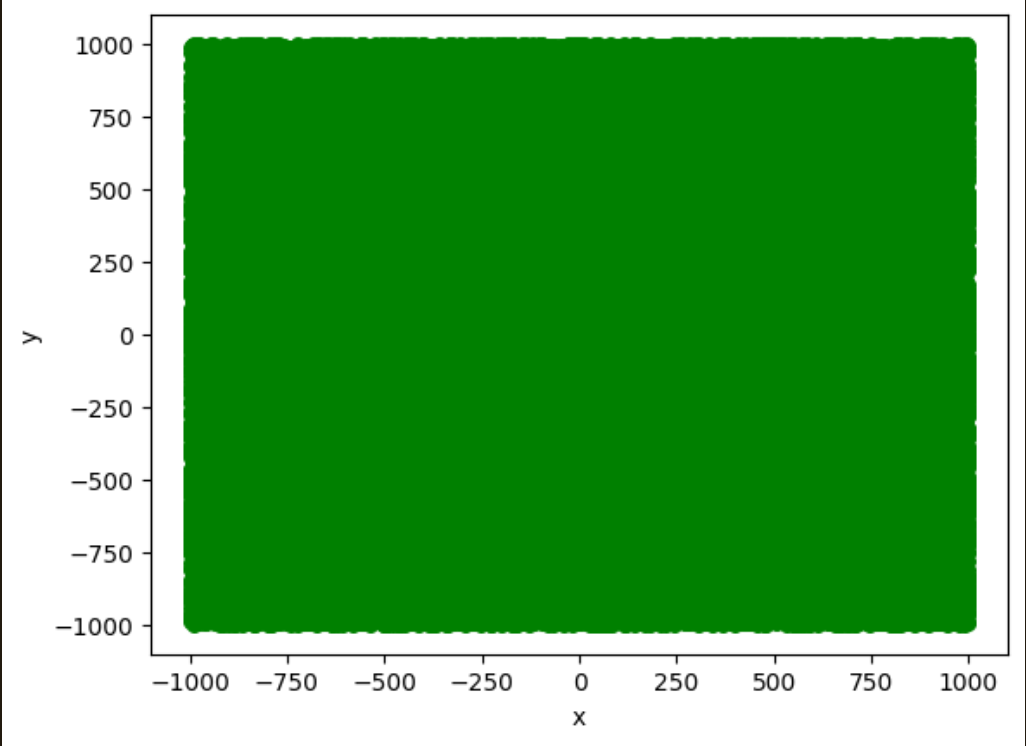
\includegraphics[width=.9\linewidth]{1.png}
      \caption*{Rys. 2}
      \label{fig:sub2}
    \end{subfigure}
    \label{fig:test}
    \end{figure}

\newpage

    \begin{figure}[!h]
    \centering
    \begin{minipage}{.5\textwidth}
      \centering
      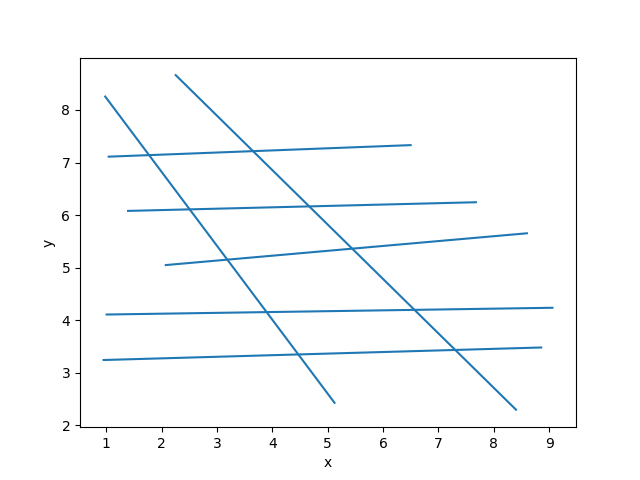
\includegraphics[width=.9\linewidth]{2.png}
      \caption*{Rys. 3}
      \label{fig:test1}
    \end{minipage}%
    \begin{minipage}{.5\textwidth}
      \centering
      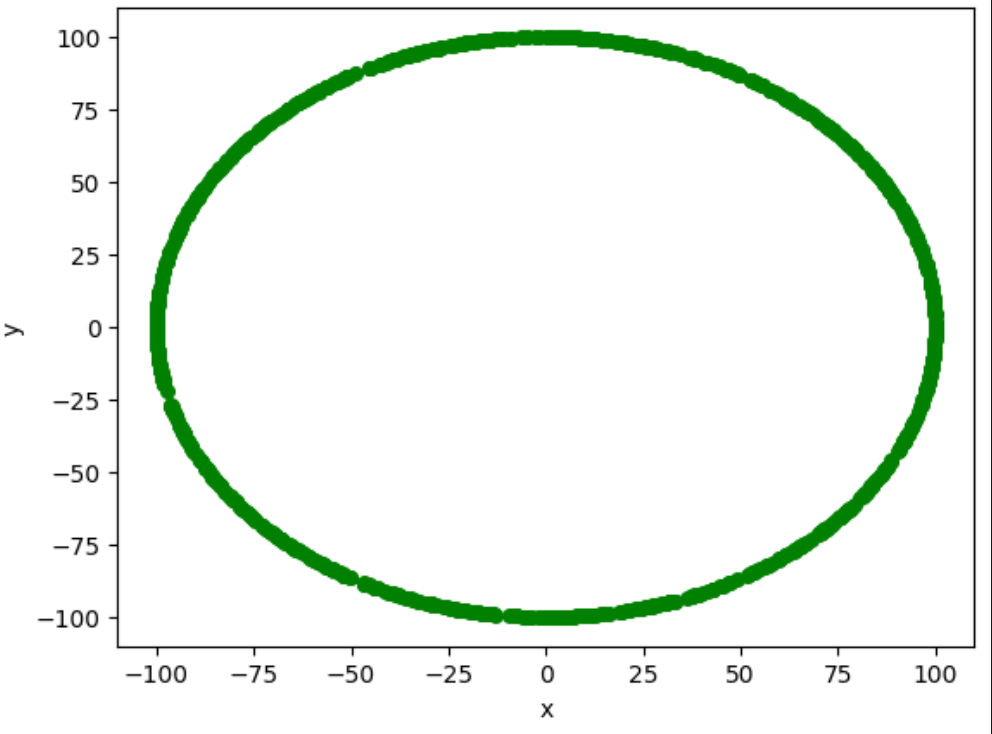
\includegraphics[width=.9\linewidth]{3.png}
      \caption*{Rys. 4}
      \label{fig:test2}
    \end{minipage}
    \end{figure}
    \begin{figure}[!h]
        \centering
        \begin{minipage}{.5\textwidth}
          \centering
          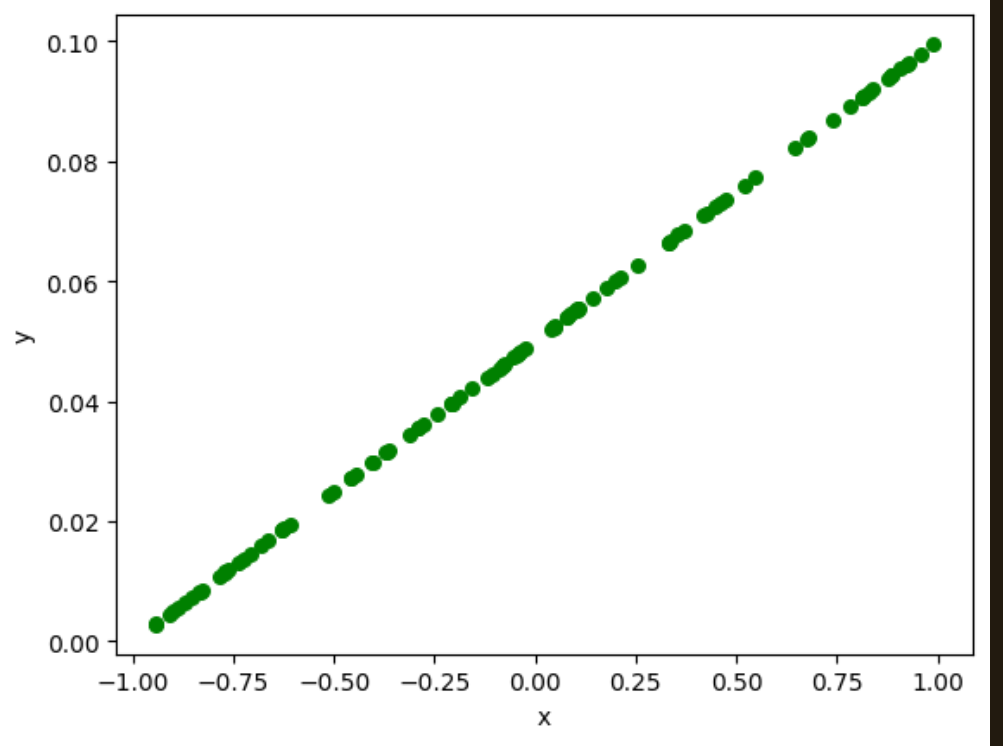
\includegraphics[width=.9\linewidth]{4.png}
          \caption*{Rys. 5}
          \label{fig:test1}
        \end{minipage}%
        \begin{minipage}{.5\textwidth}
          \centering
          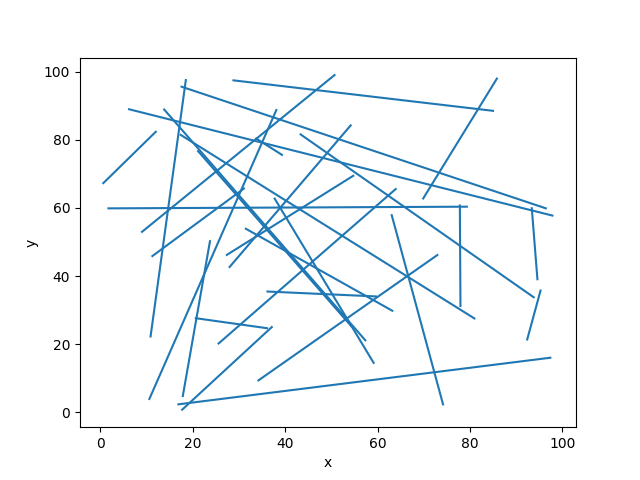
\includegraphics[width=.9\linewidth]{5.png}
          \caption*{Rys. 6}
          \label{fig:test2}
        \end{minipage}
        \end{figure}